\documentclass[12pt,twoside]{article}
\usepackage{jmlda}
\usepackage{graphicx}
\usepackage{enumerate}
\usetikzlibrary{matrix,positioning}
\usepackage[]{tikz-3dplot}
\usepackage[noend]{algorithmic}
%\renewcommand{\baselinestretch}{1. 5}

\begin{document}

\title{Использование графического процессора NVIDIA для глубокого обучения искусственных нейросетей с использованием сервиса AWS}
\thanks{Работа выполнена при поддержке РФФИ, проект 16-37-00488}
\abstract{
\emph{Abstract}. 	
В работе исследуется возможность обучения нейронной сети на процессоре графического ускорителя. Проводится анализ зависимости ошибки классификации от количества параметров и размера обучающей выборки. Рассматривается алгоритм классификации, основанный на искусственных нейросетях глубокого обучения, где под глубоким обучением понимается суперпозиция моделей. В качестве исследуемой структуры сети рассматривается композиция ограниченной машины Больцмана, автокодировщика и softmax-сети.  В работе рассматривается задача классификации временных рядов, т.е. упорядоченных по времени измерений некоторой величины.


\emph{Keywords}:
    Классификация временных рядов, Theano, Amazon Web Services, RBM, Autoencoder, CUDA.
}

\maketitle


\section{Введение}
В работе рассматривается задача классификации временных рядов, где
под временным рядом понимается упорядоченный по времени набор изменения некоторой случайной величины. В данной работе для решения этой задачи используются методы глубокого обучения. Под глубоким обучением понимается область машинного обучения, заключающаяся в построении нелинейной модели распознавания, каждый элемент которой описывает соответствующий уровень признакового агрегирования данных~\cite{foundamentals}.

Существует ряд работ~\cite{ts1,ts2,ts3}, посвященных классификации временных рядов с использованием методов глубокого обучения. В работе~\cite{ts2} используется рекуррентные нейронные сети, т.е. искусственные нейронные сети, циклические связи~\cite{foundamentals}. В работе~\cite{ts3} для классификации временных рядов рассматриваются различные комбинации ограниченной машины Больцмана, автокодировщика и двухслойной нейронной сети. В данной работе также исследуется модель, состоящая из ограниченной машины Больцмана, автокодировщика и двухслойной нейронной сети~\cite{foundamentals}.

В качестве данных для вычислительного эксперимента используются данные с акселерометра~\cite{wisdm}. Эксперимент проводится с использованием библиотеки Theano. Это библиотека для вычислений для языка Python. Theano активно используется для моделей глубокого обучения, а также для построения библиотек более высокого уровня~\cite{lasagne, pylearn}. Функции вычислений Theano компилируются, что позволяет выполнять вычисления достаточно быстро. Другой отличительной особенностью Theano является возможность использовать графического процессора с использованием архитектура параллельных вычислений CUDA. Также в экспериментальном режиме доступна возможность использовать интерфейс OpenCL, что в будущем позволит использовать для обучения нейросетей не только гарфические процессоры NVIDIA, но и других производителей. В данной работе также проводится эксперимент, направленный на сравнение эффективности обучения искусственных нейронных сетей на центральном процессоре и графическом процессоре компьютера. Эксперимент проводится с использованием сервиса облачных вычислений Amazon Web Serviece.

\section{Формальная постановка задачи}
Пусть задана выборка $\mathfrak{D} = \{(\mathbf{x}_i,y_i\}, i = 1,\dots,N$, состоящая из множества пар ``объект-ответ'', $\mathbf{x}_i \in \mathbb{R}^n$. Каждый объект принадлежит одному из $M$ классов, $y_i \in \mathbf{Y} = \{1,\dots,M\}$.

<<<<<<< .mine
%Моделью классификации $f$ назовем суперпозицию функций:
%\[
%    f(\mathbf{x},\mathbf{w}) =  \mu_1(\mu_2(\dots \mu_K(x))): \mathbb{R}^n \to [0,1]^M,
%\]
%где $\mu_k, k \in \{1,\dots,K\}$ --- модели из класса нейронных сетей, $\mathbf{w}$ --- вектор параметров данных моделей.
=======
Моделью классификации $f$ назовем суперпозицию функций:
\[
    f(\mathbf{x},\mathbf{w}) =  \mu_1(\mu_2(\dots \mu_K(x))): \mathbb{R}^n \to [0,1]^M,
\]
где $\mu_k, k \in \{1,\dots,K\}$ --- модели из класса нейронных сетей, $\mathbf{w}$ --- вектор параметров данных моделей. 
>>>>>>> .r10356

$r$-ю компоненту вектора $f(\mathbf{x},\mathbf{w})$ будем интерпретировать как вероятность отнесения объекта $\mathbf{x}_i$ к классу $r$.

Требуется минимизировать функционал ошибки $S$ на обучающей выборке $\mathfrak{G}$:
\[
    \hat{\mathbf{w}} = \argmin_\mathbf{w} S(\mathbf{w}|\mathfrak{G}),
\]
\[
    S(\mathbf{w}|\mathfrak{G}) = -\sum_{\mathbf{x},y \in \mathfrak{G} } \sum_{r=1}^M [y_i = r] \text{log} p(y=r|\mathbf{x},\mathbf{w}),
\]
где $S$ --- сумма отрицательных логарифмов правдоподобия~\cite{nnl} по всем объектам выборки.


\subsection{Структура сети}
Предлагается использовать в качестве алгоритма решения задачи нейросеть, состоящую из трех основных компонент:
ограниченной машины Больцмана, автокодировщика и двухслойной нейросети с softmax-классификатором.
\paragraph{Ограниченная машина Больцмана}
Ограниченная машина Больцмана --- это стохастическая нейросеть~\cite{rbm}, представляющая собой двудольный граф. Под стохастической нейросетью понимается сеть, содержащая в модели случайную величину. Первая доля графа соответствует нейронам входного слоя. Вторая доля соответствует скрытым нейронам, принимающим значения из множества $\{0,1\}$.

Рассмотрим простейший случай, когда входные нейроны также  принимают бинарные значения. Определим энергию пары входного слоя нейронов $\mathbf{v}$ и скрытого слоя $\mathbf{h}$ следующим образом:
\[
    E(\mathbf{v},\mathbf{h}) = -\sum_{v_l \in \mathbf{v}}b_l^v v_l -\sum_{h_j \in \mathbf{h}}b_j^h v_j - \sum_{v_l \in \mathbf{v}, h_j \in \mathbf{h}} h_j v_l w_{jl},
\]
где $w_{jl}, b^v_l, b^h_j$ --- параметры модели.

Задача тренировки ограниченной машины Больцмана предполагает максимизацию следующего функционала:
\[
\hat{\mathbf{w}},\hat{\mathbf{b}^h},\hat{\mathbf{b}^v} = \argmax_{\mathbf{w}, \mathbf{b}^h, \mathbf{b}^v} \prod_{\mathbf{x} \in \mathfrak{G}} e^{-E(\mathbf{v(\mathbf{x})},\mathbf{h(\mathbf{x})})}.
\]
В данной работе используется модифицированная версия ограниченной машины Больцмана, позволяющая работать с небинарными входными данными~\cite{gbrbm}. Для тренировки сети используется алгоритм, описанный в~\cite{foundamentals}.

\paragraph{Автокодировщик}
Автокодировщик --- это нейросеть, предназначенная для снижения размерности данных.
В просотом случае автокодировщик представляет собой суперпозицию кодирующего и декодирующего блока~\cite{foundamentals}:
\[
    \mathbf{\mu}_\text{AE} = \mathbf{\phi}(\mathbf{g}(\mathbf{x})),
\]
где $\mathbf{g}(\mathbf{x}) = \mathbf{\sigma}(\mathbf{W}_e\mathbf{x}+\mathbf{b}_e)$ --- кодирующий блок, \\
$ \mathbf{\phi}(\mathbf{g}(\mathbf{x}))  = \mathbf{\sigma}(\mathbf{W}_d\mathbf{g}(\mathbf{x})+\mathbf{b}_d)$ --- декодирующий блок, $\mathbf{\sigma}(\mathbf{t}) = \frac{1}{1+e^{-\mathbf{t}}}$ --- сигмоидная функция, $\mathbf{W}_e,\mathbf{W}_d,\mathbf{b}_e, \mathbf{b}_d$ --- параметры модели.

Введем дополнительное ограничение на матрицы $\mathbf{W}_e, \mathbf{W}_d$:
\[
    \mathbf{W}_e = \mathbf{W}_d^T.
\]

Настройку параметров модели будем проводить таким образом, чтобы по образу, получаемому с помощью кодирующего блока можно было получить вектор, близкий к исходному входному при помощи преобразования декодирующего блока:
\[
    \hat{\mathbf{W}}_e,\hat{\mathbf{W}}_d,\hat{\mathbf{b}}_e, \hat{\mathbf{b}}_d = \argmin_{\mathbf{W}_e,\mathbf{W}_d,\mathbf{b}_e, \mathbf{b}_d} \frac{1}{|\mathfrak{G}|}\sum_{\mathbf{x} \in \mathfrak{G}} ||\mu(\mathbf{x})-\mathbf{x}||^2_2.
\]
Существует ряд модификаций автокодировщика, используемых для повышения качества образов кодирующего блока. Так, в denoising-автокодировщиках на вход подаются зашумленные данные, таким образом автокодировщику требуется не только восстановить данные, но и очистить их от шума. В sparse-автокодировщика вводится дополнительный параметр, регулирующий среднюю частоту активации нейронов в сети.

\paragraph{Двухслойная нейросеть}
Двухслойная сеть представляет собой отображение~\cite{sm}:
\[
    \mathbf{a}(\mathbf{x}) = \mathbf{W}^T_2 \textbf{tanh}(\mathbf{W}^T_1 \mathbf{x}),
\]
\[
    \mathbf{\mu}_\text{softmax}(\mathbf{x}) =  \frac{\textbf{exp}(\mathbf{a}(\mathbf{x}))}{\sum_{j=1}^M \text{exp}({a}_j(\mathbf{x}))}.
\]

$r$-ю компоненту вектора $\mathbf{\mu}_\text{softmax}(\mathbf{x})$ можно интерпретировать как вероятность принадлежности объекта $\mathbf{x}$ классу $r$. Итоговая функция классификации выбирает класс объекта, соответствующий наибольшей вероятности:
\[
    f(\mathbf{x}) = \argmax_r \mu_\text{softmax}(\mathbf{\mu}_\text{AE}(\mathbf{\mu}_\text{RBM}(\mathbf{x})),
\]
где $\mathbf{\mu}_\text{softmax},\mathbf{\mu}_\text{AE}, \mathbf{\mu}_\text{RBM}$ --- двухслойная нейронная сеть, автокодировщик и ограниченная машина Больцмана соответственно.

В данной работе для тренировки сети  использовался алгоритм обратного распространения ошибок с настройкой параметров не только двухслойной сети, но и предыдущих слоев (т.н. fine-tuning~\cite{fine}):
\[
    \hat{\mathbf{\Theta}} = \argmin\sum_{\mathbf{x},y \in \mathfrak{G}}\sum_{r = 1}^M[y = r]log(\mu_\text{softmax}(\mathbf{\mu}_\text{AE}(\mathbf{\mu}_\text{RBM}(\mathbf{x}))),
\]
где $\mathbf{\Theta}$ --- параметры ограниченной машины Больцмана, автокодировщика и двухлойной сети.


\section{Запуск алгоритма на Amazon Web Services}
В данном разделе кратко изложен порядок действий для запуска вычислительного эксперимента на платформе Amazon Web Services.
\paragraph{Необходимое программное обеспечение}
Для запуска алгоритма на AWS предварительно следует установить следующие утилиты -- PUTTY (ссылка), PUTTYGen (ссылка) и либо scp (ссылка) (для Linux Mac OS), либоа WinSCP (ссылка) (для Windows).
\paragraph{Регистрация на AWS}
Далее необходимо зарегистрироваться на Amazon Web Services (ссылка). При регистрации потребуется ввести номер телефона, а также данные банковской карты, содержащей в свободном доступе 1\$, требуемый для подтверждения корректности введенных банковских данных. Активация аккаунта может занимать до 24 часов. В случае, если по прошествии этого времени активация аккаунта не удалась, рекомендуется следовать инструкциям, описанным на сайте~\cite{bank}.
\paragraph{Настройка экземпляра}
После авторизации на странице профиля Amazon WS следует зайти в консоль управления~\cite{console} и выбрать пункт <<EC2>>. На странице браузера откроется подраздел <<EC2 Dashboard>>. Для настройки нового экземпляра машины Amazon WS следует нажать кнопку <<Launch Instance>> из этого подраздела. После этого в новом окне будет доступен выбор настроек экземпляра. Для запуска вычислительного эксперимента на Theano необходимо зайти во вкладку <<Community AMIs>> и в строке поиска ввести имя конфигурации и нажать кнопку <<Select>>. В данной работе использовалась конфигурация <<ami-1797eb27>>, являющаяся версией операционной системы Ubuntu с предустановленным пакетом Theano (Рис.\ref{fig:ami}).

\begin{figure}[tb!]
  \centering
      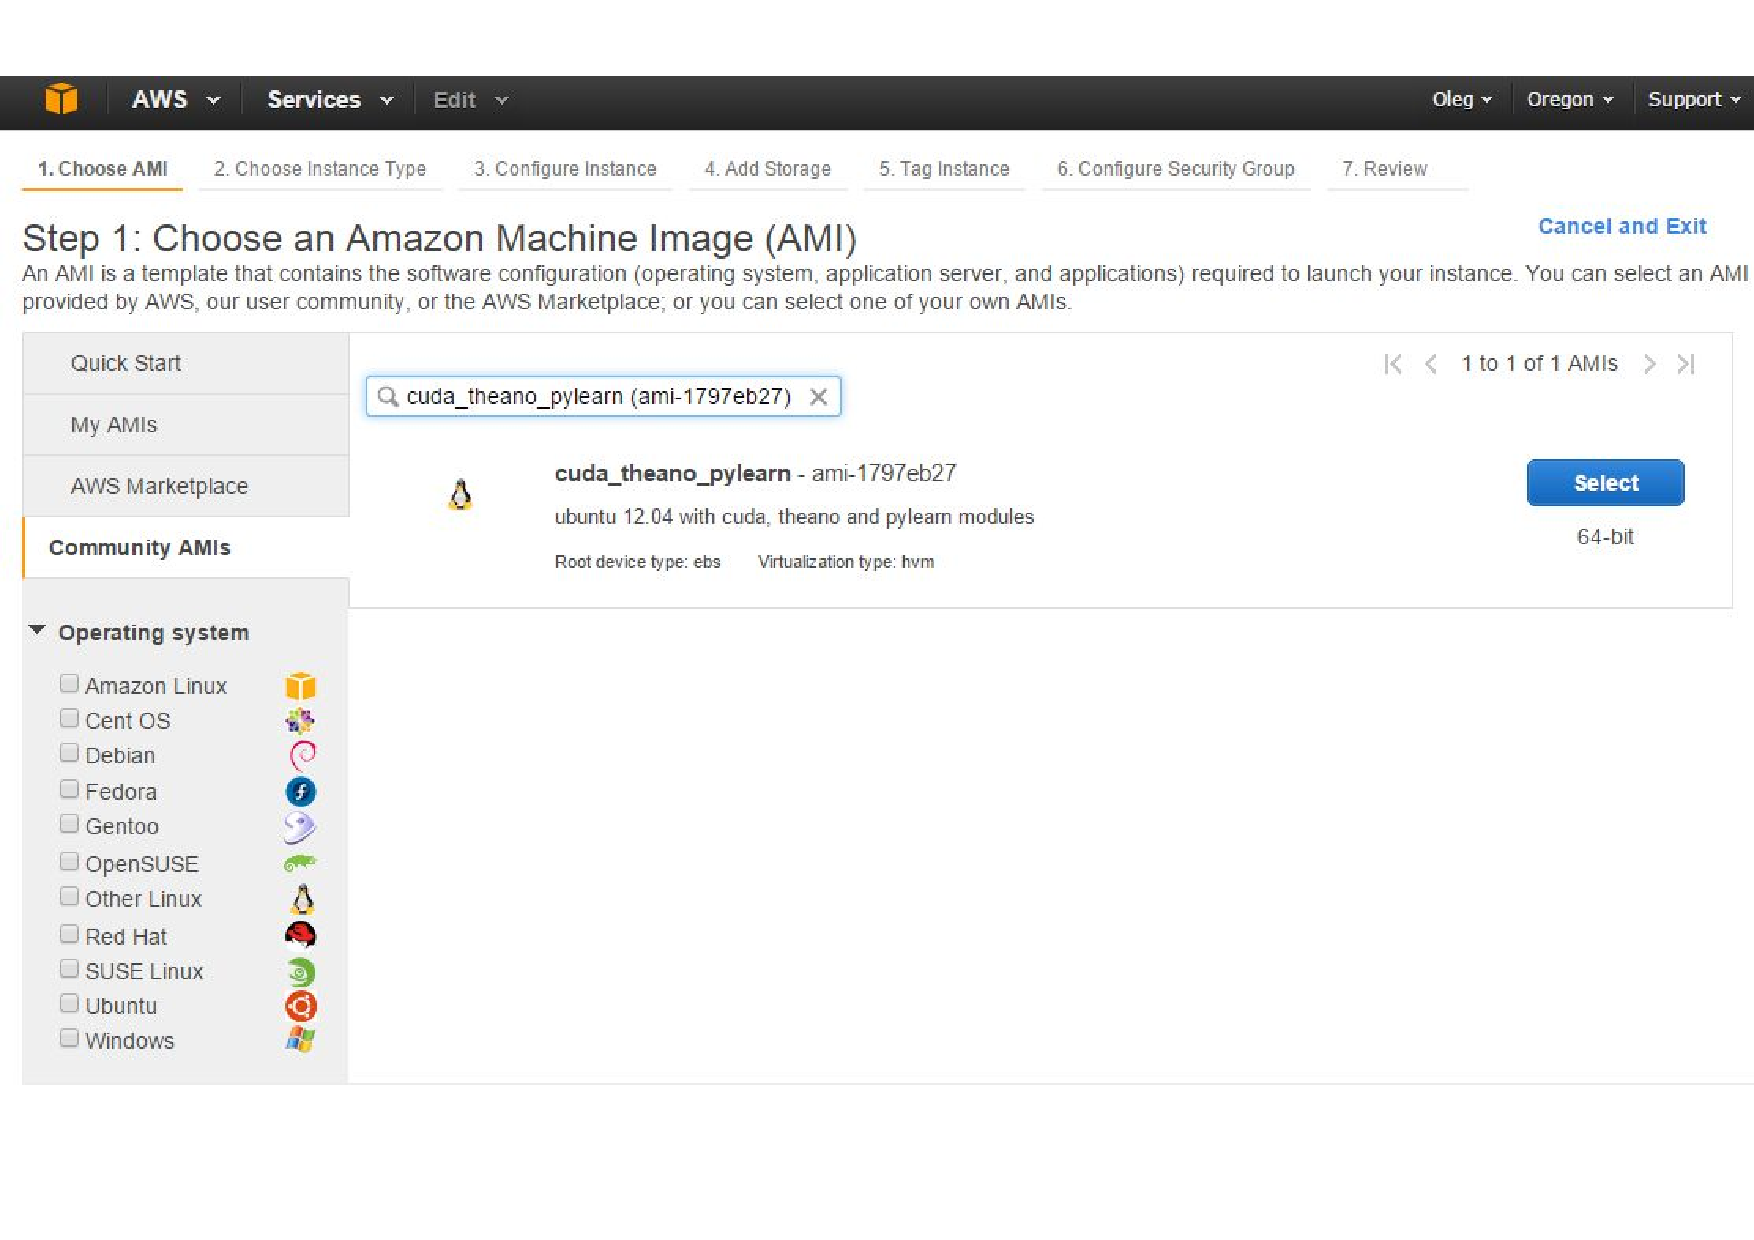
\includegraphics[totalheight=8cm]{ami.pdf}
  \caption{Выбор конфигурации в консоли Amazon Web Service}
  \label{fig:ami}
\end{figure}

После выбора конфигурации операционной системы потребуется выбрать тип экземпляра, включающий в себя такие характеристики как объем жесткого диска, объем оперативной памяти, скорость сети, наличие графического ускорителя и т.п. Для этого необходимо выделить экземпляр с подоходящими параметрами и нажать кнопку <<Review and Launch>>. После нажатия этой кнопки откроется окно с обзором параметров выбранного экзампляра. На этом этапе можно поменять параметры, вернувшись на несколько шагов назад. Если все параметры указаны верно, то необходимо нажать кнопку <<Launch>>. Далее система предложит создать пару из открытого и закрытого ключа. Для этого необходимо указать имя для пары ключей в поле <<key pair name>> и загрузить на свой компьютер файл с расширением .pem с помощью кнопки <<Download key pair>>. После завершения загрузки необходимо нажать кнопку <<Launch Instances>>. Новый экзепляр появится в подразделе <<Instances>> раздела <<EC2>>. Здесь же будет доступно описание экземпляра, в том числе и ip-адрес экземпляра (поле <<Public IP>>), необходимый для подключения к экземпляру.


\paragraph{Доступ к экземпляру}
<<<<<<< .mine
Доступ к экземпляру возможен по протоколу SSH по ip-адресу из поля <<Public IP>>.
=======
При работе с экземпляром из операционных систем Linux и Mac OS требуется изменить права для файла ключа:
\begin{quote}
chmod 400 <путь к ключу>
\end{quote}

Доступ к экземпляру можно получить по протоколу SSH по адресу, указанному системой после создания экземпляра. 
>>>>>>> .r10356
Для доступа из операционной системы Linux и Mac OS требуется ввести в консоли строку:
\begin{quote}
<<<<<<< .mine
ssh -i <путь к ключу> ubuntu@<ip-адрес>,
=======
ssh -i <путь к ключу> ubuntu@<ip-адрес>
>>>>>>> .r10356
\end{quote}
где ключ -- это файл с расширением .pem, который был ранее загружен с сайта AWS.

Для доступа из операционной системы Windows нужно использовать программы PuTTY и PuTTYgen. PuTTYgen конвертирует закрытый ключ в приемлемый для Amazon WS вид. Для конвертации ключа требуется открыть программу PuTTYgen, выбрать в программе пункт File-Load private key и выбрать полученный от Amazon WS ключ с расширением .pem. Затем требуется выбрать кнопку <<Save private key>> и сохранить полученный файл с расширением .ppk. \\
Далее необходимо открыть программу Putty и во вкладке <<Session>> в поле <<Host name (or IP adress)>> ввести строку 
\begin{quote}
ubuntu@<ip-адрес>,
\end{quote}
где ip-адрес -- это адрес из поля <<Public IP>> в описании экземпляра. Для дальнейшего использования ключа в Putty требуется выбрать вкладку Connection-SSH-Auth, нажать кнопку <<Browse>> и выбрать ppk-ключ (Рис.\ref{fig:putty}). Затем необходимо нажать кнопку <<Open>>. PuTTY выдаст окно с предупреждением, которое следует пропустить. После этого подключение к экземпляру будет установлено.

\begin{figure}[tb!]
  \centering
      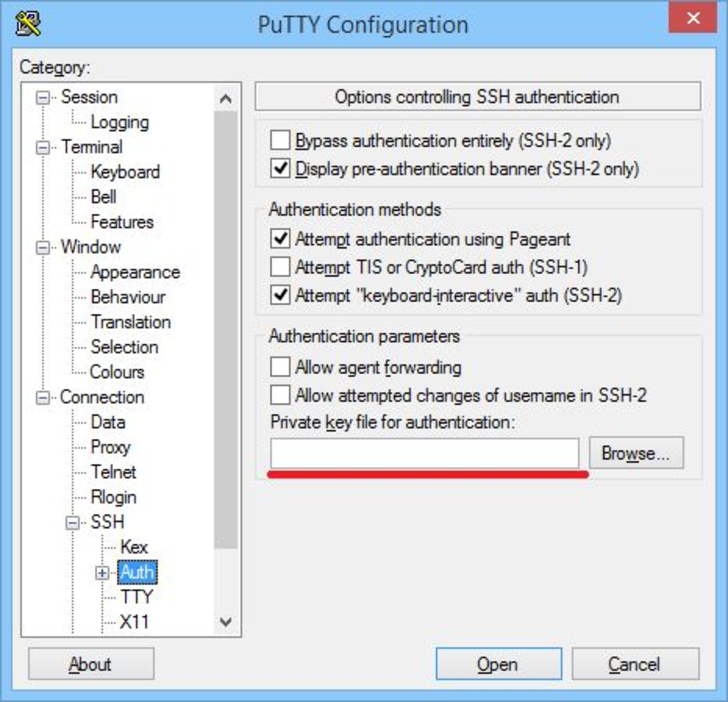
\includegraphics[height=16cm]{putty.pdf}
  \caption{Настройка аутентификации Putty}
  \label{fig:putty}
\end{figure}

\paragraph{Обмен файлами с экземпляром}
<<<<<<< .mine
Для обмена файлами с экземпляром следует использовать либо утилиту SCP для Linux и Mac OS, либо WinSCP для Windows.

В операционных системах Linux и Mac OS для копирования данных  на сервер экземпляра с использованием утилиты SCP требуется ввести в консоли строку:
=======
Для обмена файлами с экземпляром можно использовать утилиту scp для Linux и Mac OS и WinSCP для Windows. Как и в случае с соединением по SSH, при работе с экземпляром из опреационных систем Linux и Mac OS требуется изменить права для файла ключа:
\begin{quote}
chmod 400 <путь к ключу>
\end{quote}

Для копирования данных на сервер экземпляра с использованием утилиты scp требуется ввести в консоли строку:
>>>>>>> .r10356
\begin{quote}
scp -i <ключ> <локальный путь к файлу> ubuntu@<ip-адрес>:<путь к файлу на экземпляре>.
\end{quote}
Для копирования данных с сервера экземпляра  на локальный компьютер с использованием утилиты scp требуется ввести в консоли строку:
\begin{quote}
<<<<<<< .mine
scp -i <ключ> ubuntu@<ip-адрес>:<путь к файлу на экземпляре>  <локальный путь к файлу>.
=======
scp -i <путь к ключу> ubuntu@<ip-адрес>:<путь к файлу на экземпляре>  <локальный путь к файлу> 
>>>>>>> .r10356
\end{quote}
В случае копирования папки требуется добавить в команде параметр ``-r'':
\begin{quote}
scp -i <ключ> -r <локальный путь к папке> ubuntu@<ip-адрес>:<путь к папке на экземпляре> 
\end{quote}

<<<<<<< .mine
В операциинной системе Windiws для копирования данных на сервер экземпляра необходимо открыть программу WinSCP. В поле <<Host name>> нужно ввести ip-адрес <<Public IP>>, а в поле <<User name>> -- строку <<ubuntu>>. Затем требуется нажать кнопку <<Advanced>>, в новом окне выбрать вкладку
<<SSH>> - <<Authentification>>, нажать кнопку <<...>> и выбрать ppk-файл, сгенерированный PuTTYGen (Рис.\ref{fig:scp}). Затем требуется нажать кнопку <<Login>>. После этого можно передавать документы между локальным компьютером и экземпляром AWS.
=======
Для авторизации при помощи WinSCP требуется выбрать кнопку ``Advanced'', в новом окне выбрать вкладу
``SSH'' - ``Authentification'', нажать кнопку ``...'' и выбрать ppk-файл (Рис.\ref{fig:scp}). Затем требуется указать ip-адрес экземпляра в поле ``Host name'', строку ``ubuntu'' в поле ``User name'', и нажать кнопку ``Login''. После этого можно передавать документы между локальным компьютером и экземпляром AWS.
>>>>>>> .r10356
\begin{figure}[tb!]
  \centering
      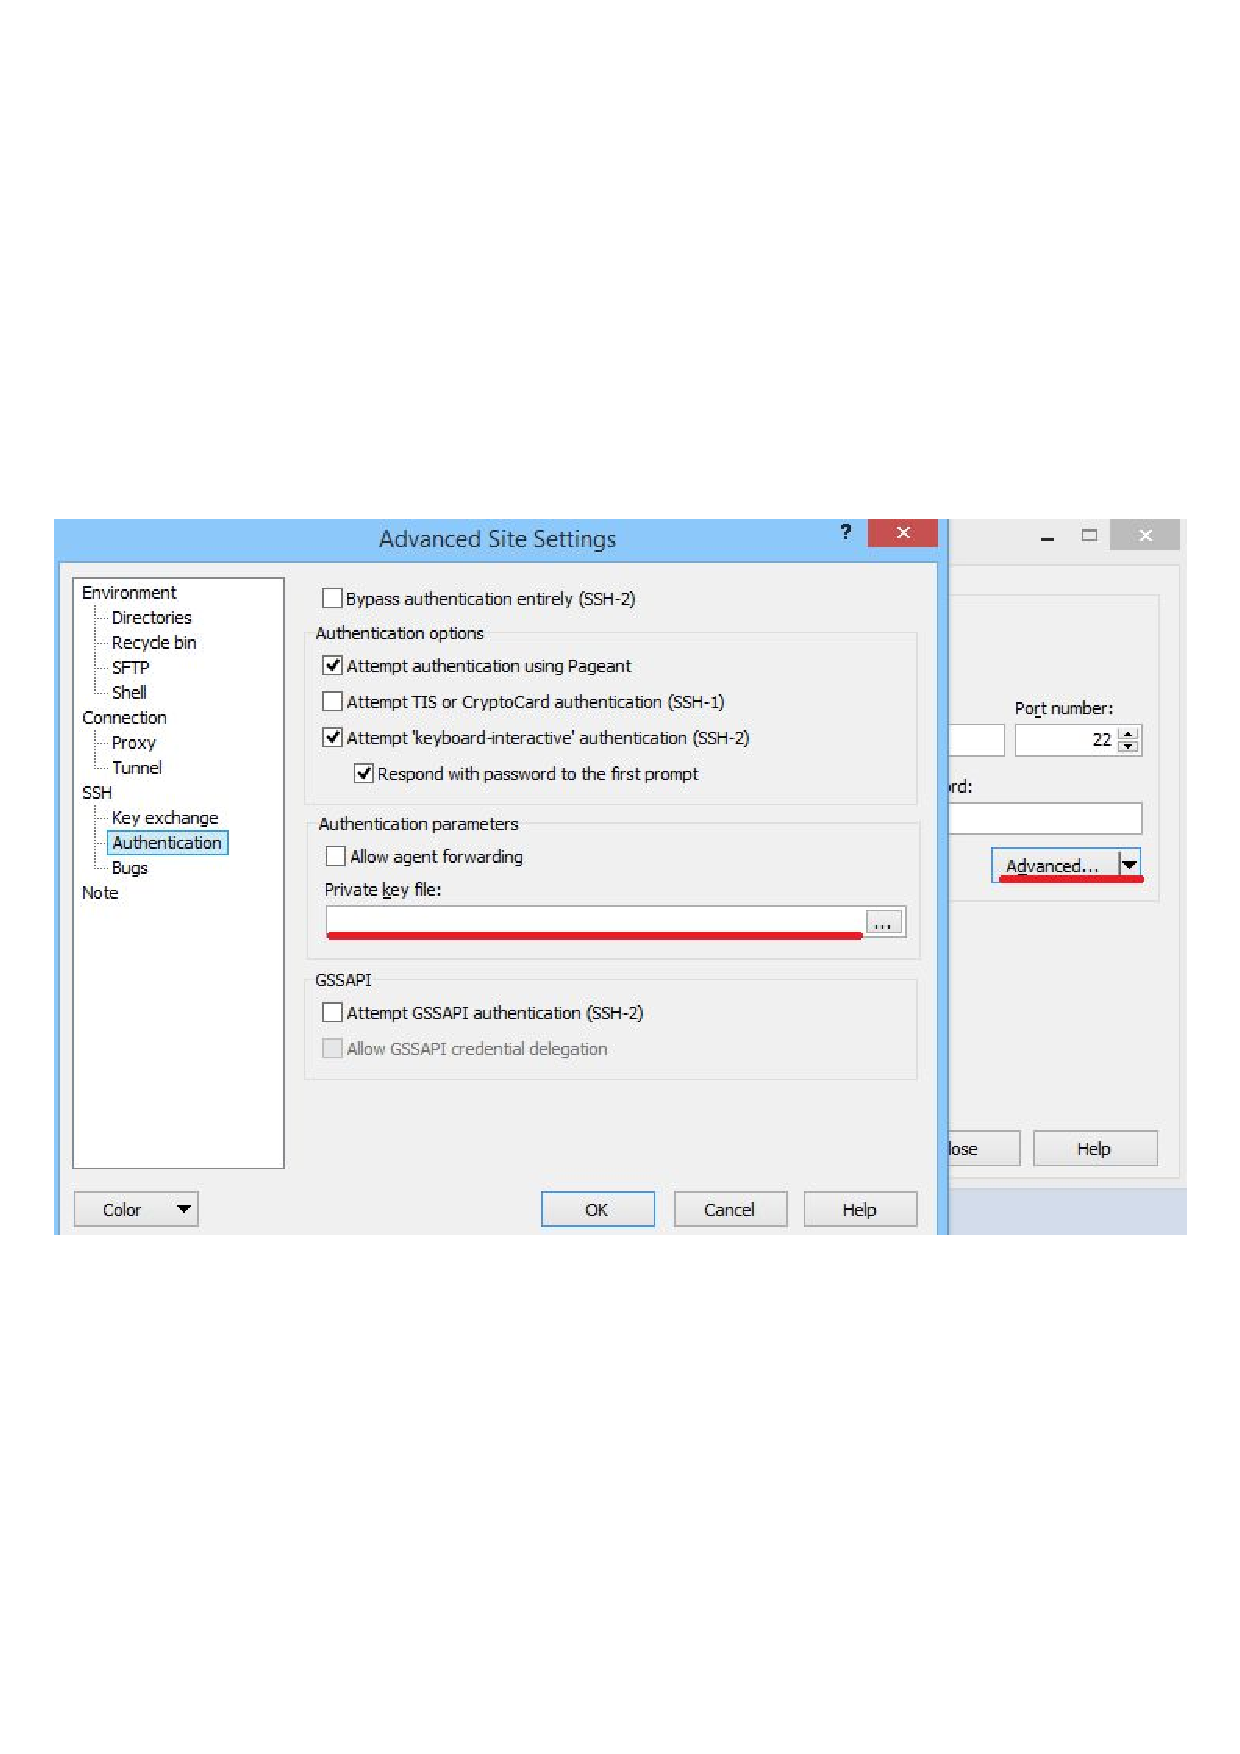
\includegraphics[height=16cm]{scp.pdf}
  \caption{Настройка аутентификации WinSCP}
  \label{fig:scp}
\end{figure}

\paragraph{Завершение работы с экземпляром}
По завершению работы с экземпляром требуется уничтожить его, выбрав его в консоли управления, и выбрав команду ``Terminate''. Стоит отметить, что в консоли также имеется команда <<Stop>>, отключающая экземпляр. Но за хранение данных на отключенном экземпляре может также взиматься дополнительная плата. Также рекомендуется удалить все хранилища данных, присоединенные к экземпляру (вкладка <<Volumes>>).

\paragraph{Запуск вычислительного эксперимента}
Для запуска вычислительного эксперимента с использованием Theano требуется указать параметры конфигурации Theano перед запуском. В противном случае, будет принята конфигурация по умолчанию. Наиболее простым вариантом установки параметров Theano является вызов программы с использованием следующего синтаксиса:
\begin{quote}
THEANO\_FLAGS=<параметры Theano в формате ``ключ=значение'' через запятую> python <путь к скрипту>
\end{quote}

Для запуска скрипта с $n$ процессорами требуется вызвать его следующим образом:
\begin{quote}
OMP\_NUM\_THREADS=n python <путь к скрипту>
\end{quote}

Для запуска скрипта с использованием CUDA требуется вызвать скрипт следующей командой:
\begin{quote}
THEANO\_FLAGS=device=gpu,floatX=float32 python <путь к скрипту>
\end{quote}
Здесь ``floatX=float32'' --- параметр, отвечающий за формат вещественных чисел при обработке Theano. В настоящее время поддерживается только float32.

\paragraph{Общий план запуска алгоритма}
Ниже приведен общая пошаговая инструкция запуска алгоритма на сервере AWS:
\begin{itemize}
\item Зарегистрироваться на AWS
\item Сконфигурировать экземпляр
\item Скопировать код и данные проекта на сервер (например, в папку /home/ubuntu/)
\item Присоединиться к серверу по протоколу ssh
\item Зайти в папку с проектом с использованием команды cd
\item Запустить вычислительный эксперимент.
\item Уничтожить экземпляр

В качестве примера запуска вычислительного эксперимента, можно вызвать команду:
\begin{quote}
sh run8CPU.sh
\end{quote}
для запуска эксперимента на 8 ядрах процессора или
\end{itemize}
\begin{quote}
sh runGPU.sh
\end{quote}
для запуска эксперимента на графическом ускорителе. Подробно параметры запуска описаны в Readme-файле проекта.
\section{Вычислительный эксперимент}
В качестве данных для проведения вычислительного эксперимента использовались данные WISDM~\cite{wisdm}, представляющие собой набор записей акселерометра. Каждой записи соответствуют три координаты по осям акселерометра. Набор данных содержит записи движений для 6 классов переменной длины.
При проведение вычислительного эксперимента из каждой записи использовались первые 200 сегментов. Т.к. выборка несбалансирована, в выборку добавлялись повторы записей классов, содержащих количество записей, меньшее чем у большего класса.

Для оценки качества классификации была проведена кросс-валидация в соотношении количества объектов обучающей и контрольной выборки 3:1. Количество нейронов на каждом слое рассчитывалось из соотношения 10:6:3. При кросс-валидации для каждого отсчета количества нейронов было произведено 5 запусков. При обучении двухслойной нейронной сети проводился мультистарт~\cite{multi}, т.е. одновременный запуск обучения сети с 8 разными стартовыми значениями параметров для предотвращения возможного застревания алгоритма обучения в локальном минимуме, при оценке качества классификации выбиралась модель с наилучшими результатами. График зависимости ошибки классификации от количества нейронов изображен на Рис.~\ref{fig:neurons}.

\begin{figure}[tb!]
  \centering
      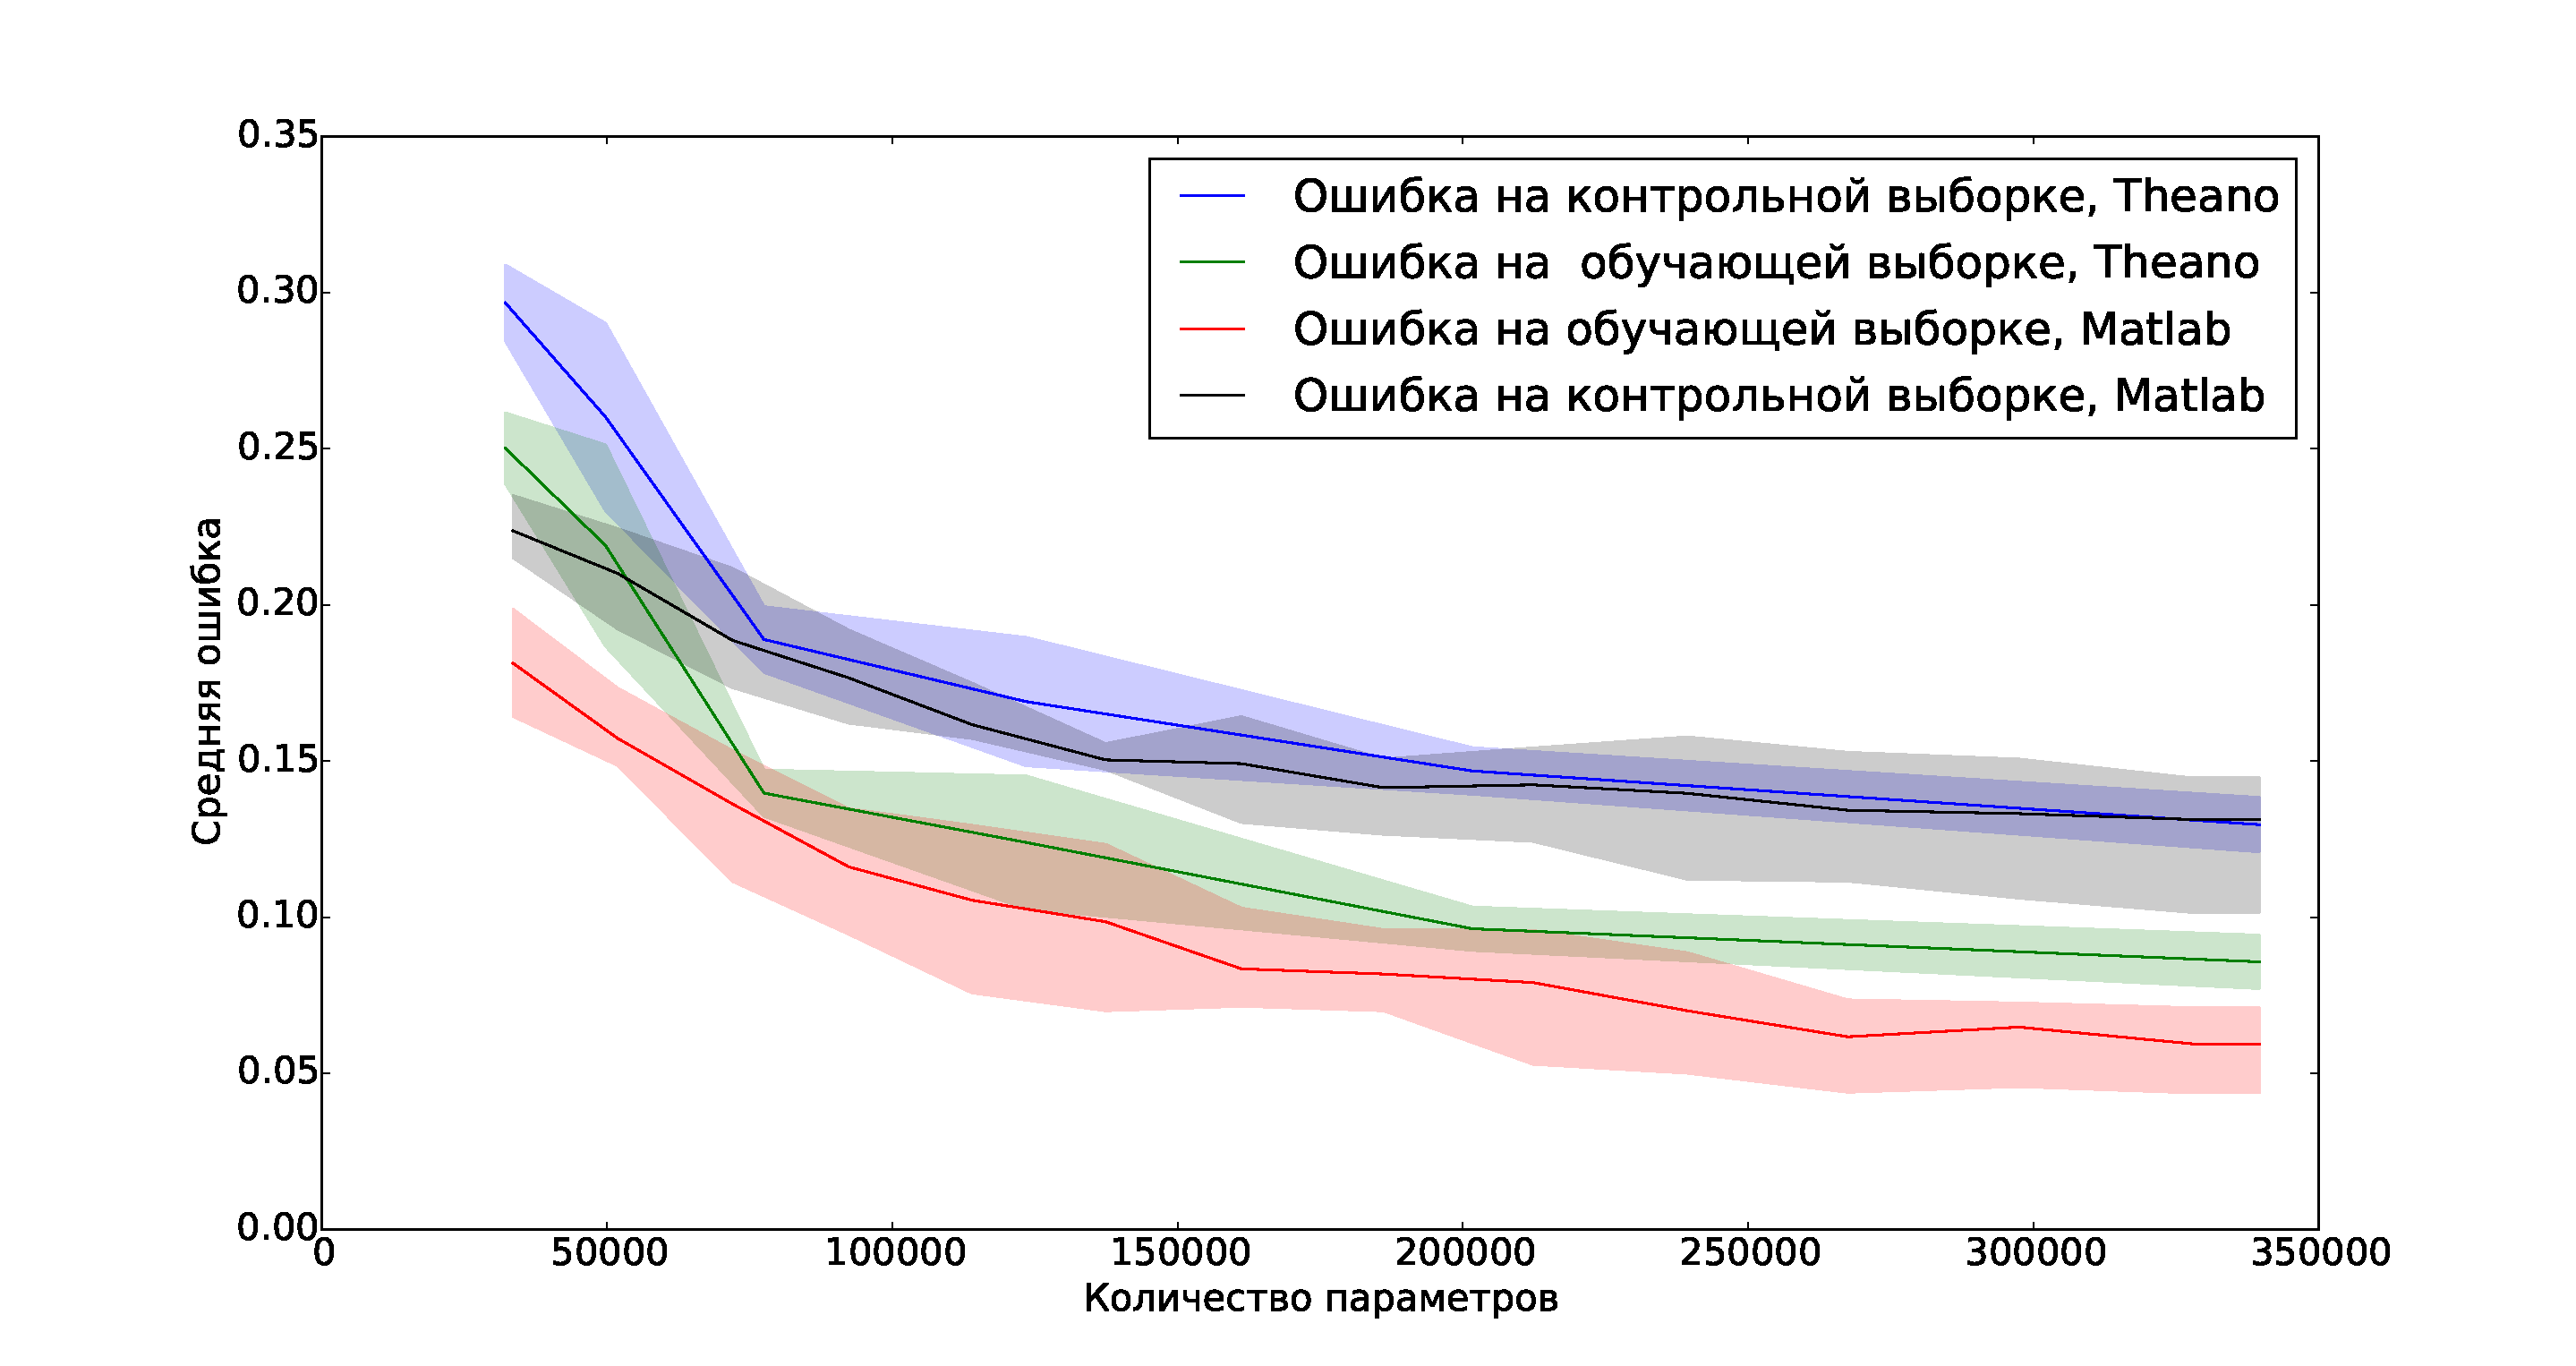
\includegraphics[width=1.0\textwidth]{neurons.pdf}
  \caption{Зависимость ошибки от количества нейронов}
  \label{fig:neurons}
\end{figure}


Для оценки зависимости качества классификации от размера обучающей выборки была проведена кросс-валидация с фиксированным количеством объектов в обучающей выборке (25\% исходной выборки) и переменным размером обучающей выборки. Количество нейронов было установлено как 378:226:113. При кросс-валидации для каждого отсчета было произведено 5 запусков. График зависимости ошибки классификации от количества нейронов изображен на Рис.~\ref{fig:samples}.



\begin{figure}[tb!]
  \centering
      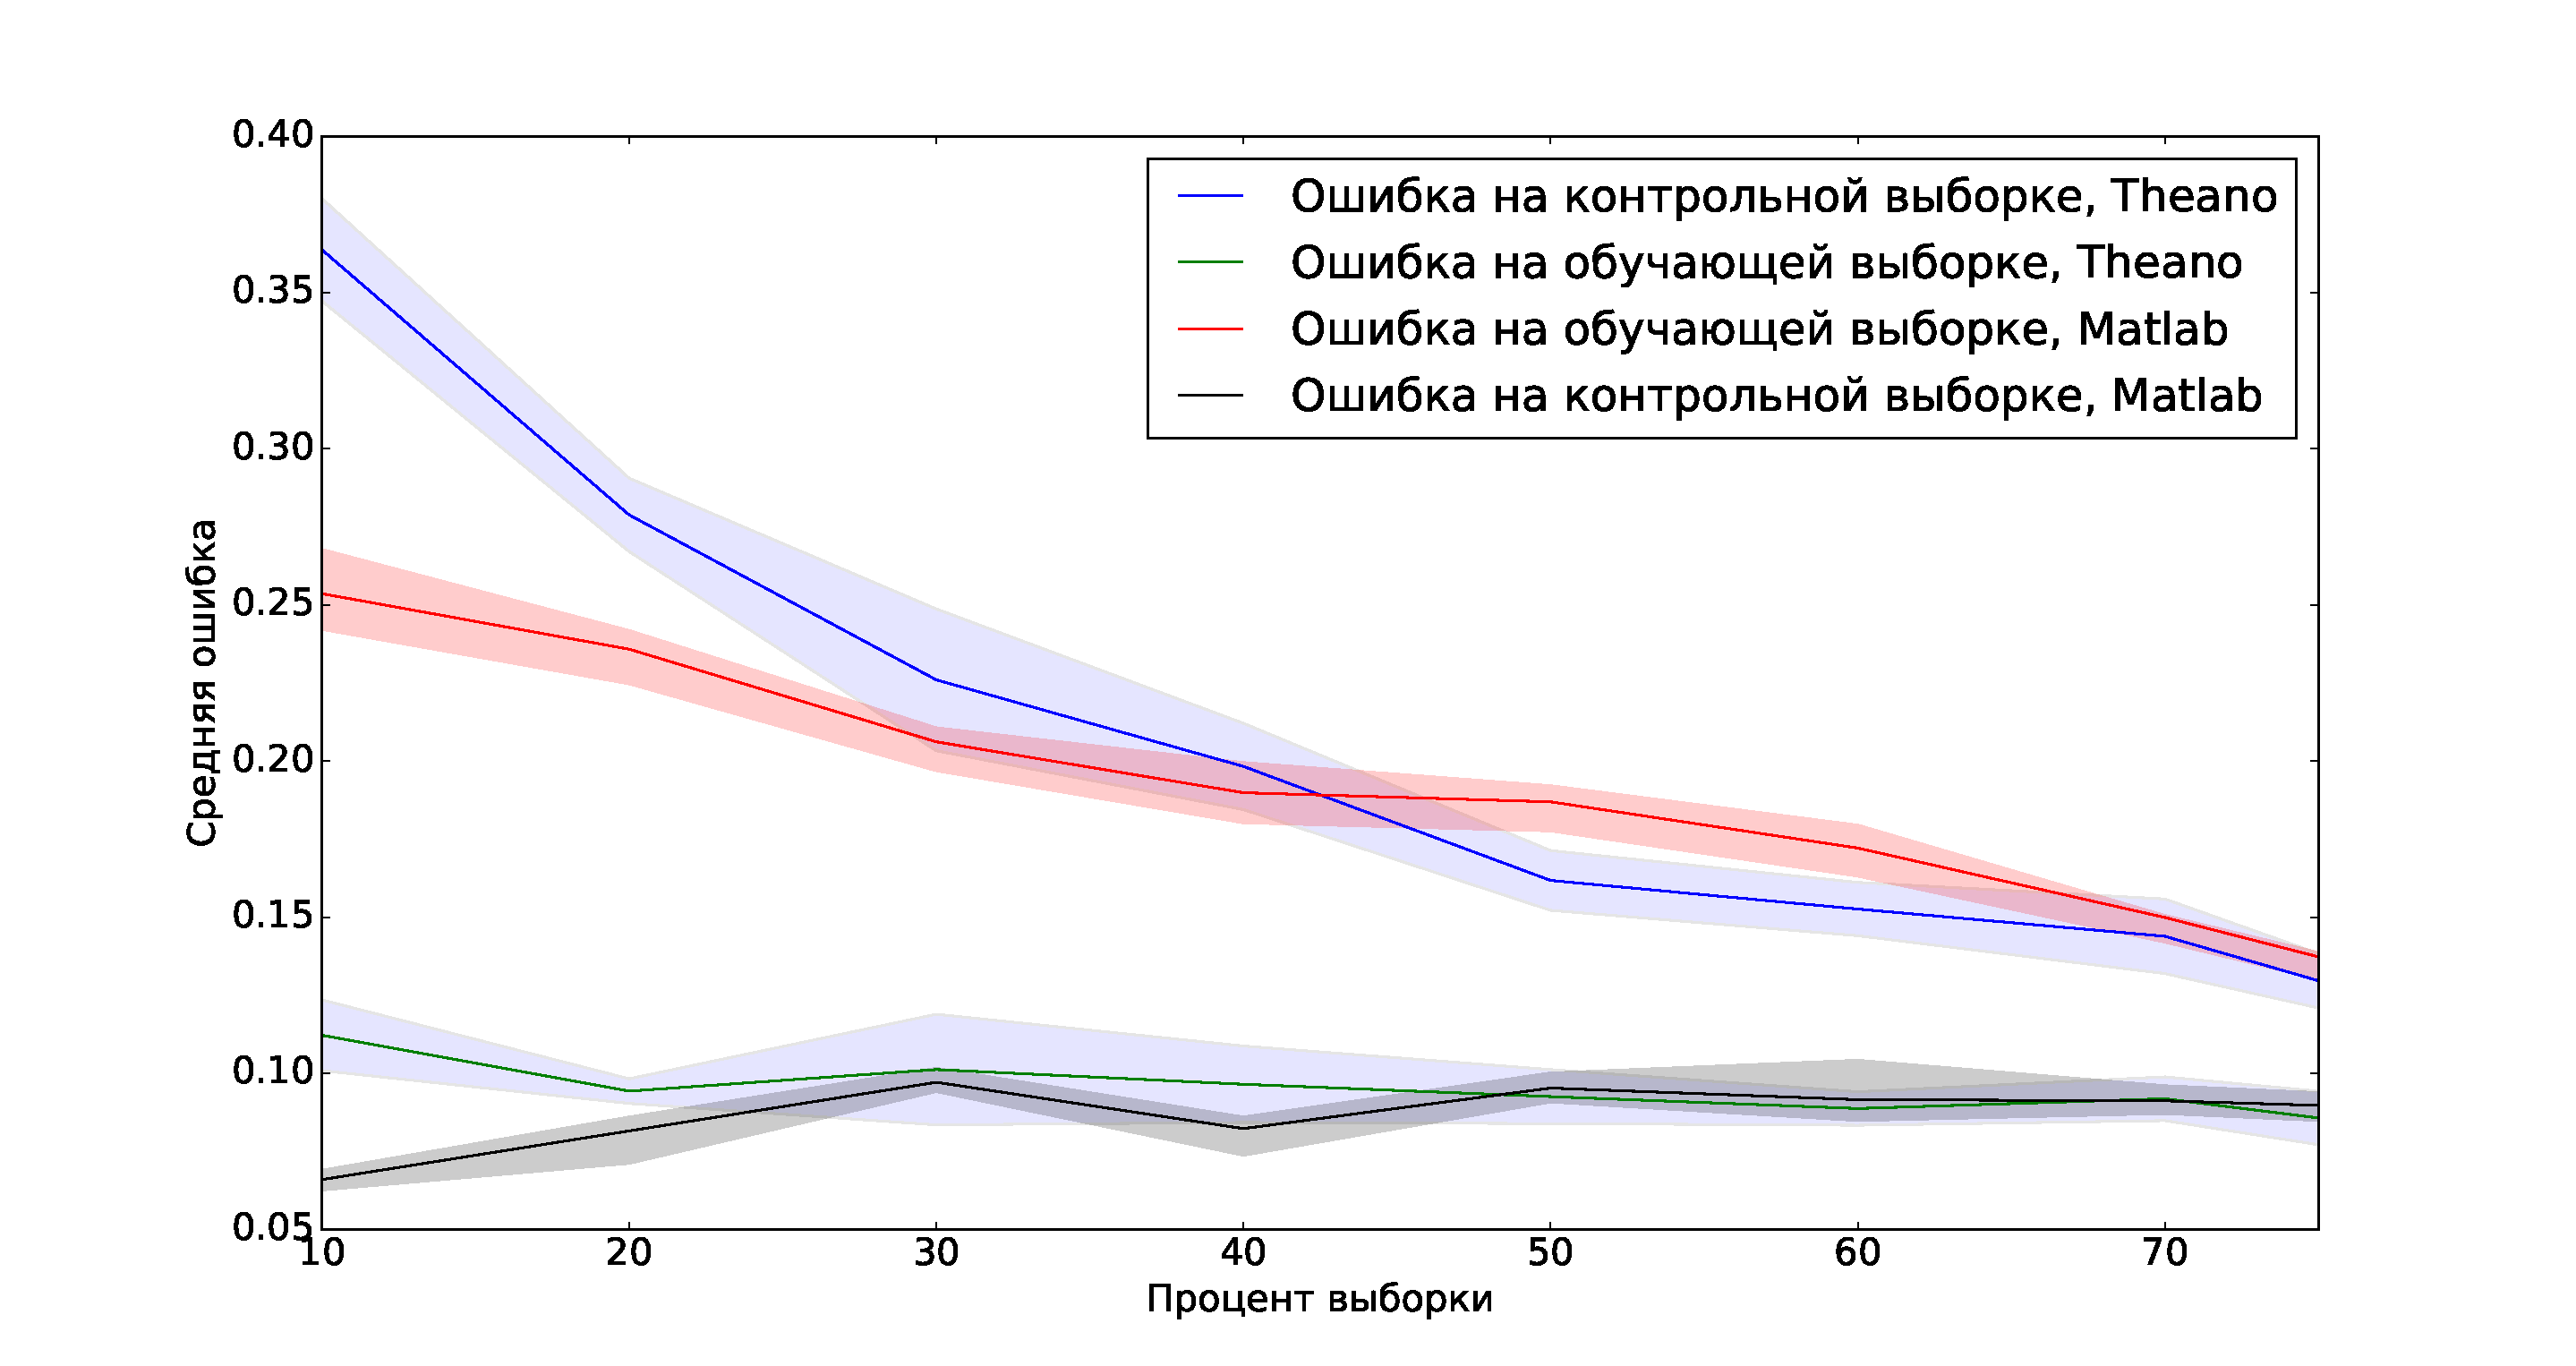
\includegraphics[width=1.0\textwidth]{samples.pdf}
  \caption{Зависимость ошибки от размера обучающей выборки}
  \label{fig:samples}
\end{figure}

Для исследования скорости работы процесса обучения нейросети в зависимости от конфигурации Theano был проведен следующий эксперимент:
проводилось обучение двухслойной нейросети на основе подсчитанных заранее параметров ограниченной машины Больцмана и автокодировщика. Обучение проходило за 100 итераций. При обучении алгоритм запускался параллельно с $n$ разными стартовыми позициями, $n \in \{1,\dots,4\}.$ Количество нейронов было установлено как 300:200:100.
Запуск осуществлялся с следующими конфигурациями Theano:
\begin{itemize}
\item вычисление на центральном процессоре, задействовано
одно ядро
\item вычисление на центральном процессоре, задействовано четыре ядра
\item вычисление на центральном процессоре, задействовано восемь ядер
\item вычисление на графическом процессоре
\end{itemize}

Результаты эксперимента приведены на Рис.~\ref{fig:speed}. Как видно из графика, вычисление с использованием CUDA показывает значительное ускорение по сравнению с вычислением на центральном процессоре.

\begin{figure}[tb!]
  \centering
      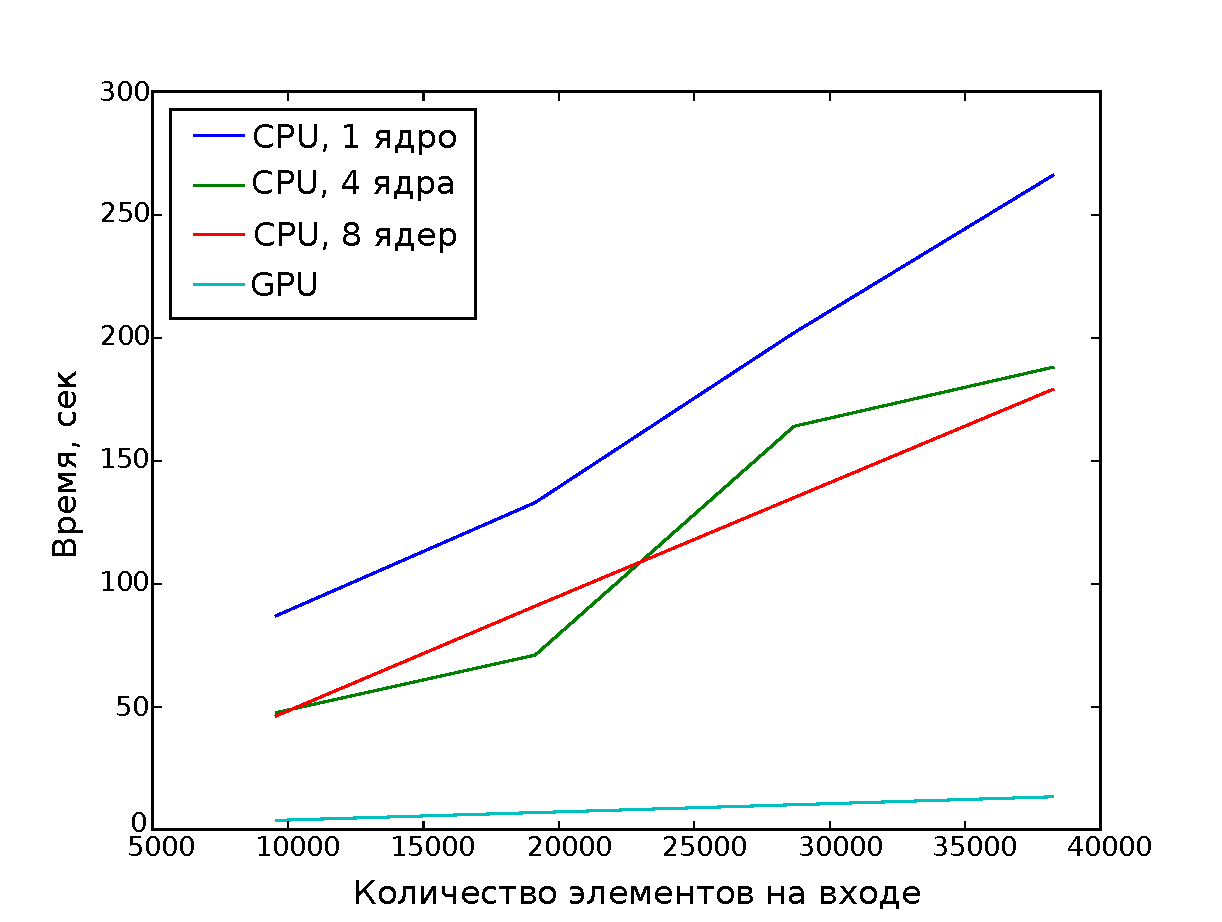
\includegraphics[width=0.8\textwidth]{result.pdf}
  \caption{Результаты эксперимента по исследованию скорости работы процесса обучения}
  \label{fig:speed}
\end{figure}

\section{Заключение}
В данной работе был проведен ряд  вычислительных экспериментов с использованием библиотеки Theano и сервисом облачных вычислений Amazon WebService. Проведены эксперименты для установления зависимости ошибки классификации временных рядов с использованием сетей глубокого обучения от размера выборки и количества параметров сети. Исследовалась эффективность обучения искусственной нейросети с использованием графического процессора. Эксперимент показал большую эффективность вычислений на графическом процессоре. Скорость обучения сети с использованием графического процессора значительно выже, чем с использованием центрального процессора. Исходный код эксперимента доступен по адресу~\cite{svn}.

Авторы выражают благодарность д. ф.-м. н. Вадиму Викторовичу Стрижову за постановку задачи и внимание к работе.
\begin{thebibliography}{1}

\bibitem{foundamentals}
    \BibAuthor{Kyunghyun Cho}
Foundations and Advances
in DeepLearning

%http://www.diva-portal.org/smash/get/diva2:710518/FULLTEXT02
\bibitem{ts1}
    \BibAuthor{Längkvist, M., Karlsson, L., Loutfi, A.}
A review of unsupervised feature learning for time-series modelling

%http://tdesell.cs.und.edu/papers/2015_evocop.pdf
\bibitem{ts2}
    \BibAuthor{Travis Desell, Sophine Clachar, James Higgins, Brandon Wild}
Evolving Deep Recurrent Neural Networks Using Ant
Colony Optimization

\bibitem{ts3}
    \BibAuthor{M. Popova, V. Strijov}
Building superposition of deep learning neural networks
for solving the problem of time series classification

\bibitem{wisdm}
\BibAuthor{Kwapisz J. R., Weiss G. M., Moore S.}
 Activity recognition using cell phone
accelerometers // SIGKDD Explorations, 2010. Vol. 12. No 2. P. 74-82.

\bibitem{pylearn}
URL://http://deeplearning.net/software/pylearn2/

\bibitem{lasagne}
URL:http://lasagne.readthedocs.org/en/latest/

%http://www.gatsby.ucl.ac.uk/~chuwei/paper/smc.pdf
\bibitem{nnl}
\BibAuthor{Kaibo Duan, S. Sathiya Keerthi, Wei Chu,Shirish Krishnaj Shevade,
Aun Neow Poo}
Multi-Category Classification by Soft-Max
Combination of Binary Classifiers

\bibitem{bank}
URL:https://aws.amazon.com/ru/billing/faqs/

%http://image.diku.dk/igel/paper/TRBMAI.pdf
\bibitem{rbm}
    \BibAuthor{Asja Fischer, Christian Igel}
Training Restricted Boltzmann Machines: An Introduction

\bibitem{stochastic}
\BibAuthor{Ruya SAMLI}
STOCHASTIC NEURAL NETWORKS AND THEIR
SOLUTIONS TO OPTIMISATION PROBLEMS

%https://users.ics.aalto.fi/praiko/papers/nips11Cho.pdf
\bibitem{gbrbm}
\BibAuthor{KyungHyun Cho, Tapani Raiko and Alexander Ilin}
Gaussian-Bernoulli Deep Boltzmann Machine

%http://www.jmlr.org/papers/volume11/vincent10a/vincent10a.pdf
\bibitem{denoise}
\BibAuthor{Pascal Vincent, Hugo Larochelle, Isabelle Lajoie, Yoshua Bengio,
Pierre-Antoine Manzagol}
Stacked Denoising Autoencoders: Learning Useful Representations in
a Deep Network with a Local Denoising Criterion

%http://web.stanford.edu/class/cs294a/sparseAutoencoder.pdf
\bibitem{sparse}
URL:http://web.stanford.edu/class/cs294a/sparseAutoencoder.pdf


%http://www.mitpressjournals.org/doi/pdf/10.1162/neco.2006.18.7.1527
\bibitem{sm}
\BibAuthor{Geoffrey E. Hinton,Simon Osindero,
Yee-Whye Teh}
A Fast Learning Algorithm for Deep Belief Nets



%http://jmlr.org/papers/volume11/erhan10a/erhan10a.pdf
\bibitem{fine}
\BibAuthor{Dumitru Erhan,
Yoshua Bengio,
Aaron Courville,
Pierre-Antoine Manzagol,
Pascal Vincent}
Why Does Unsupervised Pre-training Help Deep Learning?

\bibitem{console}
URL:https://us-west-2.console.aws.amazon.com/console/

%URL:http://www.researchgate.net/profile/Marco_Locatelli/publication/227102777_Machine_learning_for_global_optimization/links/0c96053b561d2cf6c1000000.pdf
\bibitem{multi}
\BibAuthor{Andrea Cassioli,D. Di Lorenzo,Marco Locatelli,Fabio Schoen,Marco Sciandrone}
Machine Learning for Global Optimization

\bibitem{svn}
URL:https://svn.code.sf.net/p/mlalgorithms/code/Group074/Bakhteev2015TheanoCuda/code/
\end{thebibliography}


\end{document}
